\documentclass{report}
\usepackage[utf8]{inputenc}
\usepackage[english]{babel}
\usepackage{listings}
\usepackage{graphicx}
\usepackage{bm}
\usepackage{amsmath}
\usepackage{mathtools}
\usepackage{float}
\usepackage{tabularx}
\usepackage{tikz}

\setcounter{secnumdepth}{3}

\title{Webdevelopment}
\date{}
\author{}

\begin{document}

\maketitle

\chapter{A Bird's Eye View of the Web}

\emph{Vint Cerf} invented the internet
while \emph{Tim Berners-Lee} invented the web.

\section{Dreams and visions}

\emph{Ted Nelson} coined the term hypertext.
His showpiece is his \emph{Xanadu} project.

\emph{Douglas Engelbart} gave
the \emph{Mother of All Demos} in 1968.

\section{The Web and universality}

\subsection{Origins and aims}

In 1989, Berners-Lee convinced CERN to let him work
on the Web with his \emph{Information Management: A Proposal}.
A year later, the first webpages came online.

CERN decided to make the Web available royalty-free in 1993.

Before the Web, the world was heterogenous.
It was difficult to target soft- and hardware.

In contrast, the Web strives to be \emph{universal}.
Anyone is free to build for the Web.
Although, app stores are a counterexample
to the freedom to develop for the Web.

Web technologies are standardized
by the World Wide Web Consortium (W3C)

The Web brings \emph{permissionless innovation}.
You don't need anyone's permission to launch a new idea.

\subsection{Technical foundations}

The Web is an application that runs on top of the Internet.
``The \emph{Internet} is to the \emph{Web}
what the \emph{telephone network} is to \emph{fax}.''

Examples of applications which are on the Internet,
but not on the Web:
Skype, BitTorrent, e-mail, VPN, \dots

The Web as a decentralized hypertext system
consists of simplistic one-way links.
Text and hyperlinks are contained in an HTML document.
These are \emph{not shareable}.
Styling, media and scripts are stored outside an HTML document.
These \emph{are} shareable.

These realizations contrast Ted Nelson's views.

``Individual links are allowed to break
so that the entire Web does not.'' -- Tim Berners-Lee

\section{Opportunities and challenges}

\subsection{The Web for machines}

The Web's architecture makes it hard
to locate specific content.
\emph{Crawlers} sprung into life
to index content (in a centralized manner).

\emph{RSS feeds} contain the title and summary
of the last entries on a website.
Here, the user is in control of what they are fed
and not the other way around.

The Web as it is, is designed for humans.
It is hard for machines to understand the Web.
Web APIs expose functionality to automated clients.

The Semantic Web is a layer
on top of the existing Web.
We would like that the Semantic Web
integrates into the existing Web.

In the early days of the Semantic Web,
noone built applications, because there was no data.
Noone published data, because there were no applications.

Berners-Lee proposed \emph{Linked Data}:
principles to follow to publish data semantically.
Let's just get data out and apps will follow.

\subsection{Threats to universality}

\emph{Native apps} essentially undo
all progress on device-independence.
In contrast, we need but only
a generic browser to browse the Web.

Certain browser vendors provide
software to access to the web.
A few search engine companies make or break websites.

Centralized platforms control data and identities.
Ironically, permissionless innovation enables
platforms (like Facebook) that prevent it.

\chapter{Web Architecture \& Technologies}

The Web consists of 3 separate but connected inventions.
A URL uniquely identifies a resource.
HTTP allows one to retrieve the resource identified by a URL.
An HTML document may represent a resource
or link to other resources through their URL.

\section{Core Web Standards}

\subsection{URL}

A Web URL uniquely \emph{identifies} and \emph{locates}
a resource anywhere in the universe.

A string is a unique \emph{identifier} if
at most one entity corresponds to it,
e.g. a national number uniquely identifies a person,
but does not allow locating them.

A string is a unique \emph{locator} if
at most one location corresponds to it,
e.g. a street address uniquely identifies a location,
but does not allow uniquely identifying a person.

URL became part of a family of technologies related to identification.
An example of a URL is \textit{mailto:ruben.verborgh@ugent.be},
where Ruben's mailbox is uniquely identified and located.
An example of a URN (\emph{Uniform Resource Name}) is an ISBN,
which identifies a book in a location-independent manner.
URIs (\emph{Uniform Resource Identifiers})
are a union of URLs and URNs.
IRI (\emph{Internationalized Resource Identifier})
extends URI with non-ASCII characters.

The uniform structure of an HTTP URL includes the following
\begin{center}
  \texttt{http://<host>/<path>?<query>\#<fragment>}
\end{center}
where \textbf{host} identifies the target machine,
\textbf{path} identifies the resource within the machine,
\textbf{query} optionally refines the resource and
\textbf{fragment} optionally identifies a fragment of the resource.

An HTTP URL contains instructions
to obtain a representation of a resource.
\begin{enumerate}
  \item Using DNS, the client looks up the host's IP address.
  \item The client then requests \texttt{/<path>?<query>}.
  \item The client finds \texttt{\#fragment}.
\end{enumerate}

\subsection{HTTP}

HTTP is a protocol that standardized client-server communication.
HTTP standardizes how clients \emph{request}
resource representations from servers.
HTTP standardizes how servers reply with a \emph{response}
that may contain a representation.

A client sends a request of the following form.
\begin{lstlisting}
  GET <path> HTTP/<version>
  <headers>
  <body>
\end{lstlisting}

An HTTP method is \emph{safe} if it is read-only.
Examples are GET or HEAD.

An HTTP method is \emph{idempotent} if
alterations don't alter the outcome.
Examples are any safe method, PUT or DELETE.

A client sends a \texttt{Host} header with the hostname,
so one server may host multiple websites.
There is no one-to-one mapping from hostnames to IPs,
one website may be hosted on multiple servers.
As well as one server may host multiple websites.

A server generates a response of the following form.
\begin{lstlisting}
  HTTP/<version> <status> <message>
  <headers>
  <body>
\end{lstlisting}

HTTP status codes in a nutshell.
\begin{itemize}
  \item 1xx: Hold on.
  \item 2xx: Here you go.
  \item 3xx: Go away.
  \item 4xx: You messed up.
  \item 5xx: I messed up.
\end{itemize}

\subsection{HTML}

HTML is markup language that captures the structure of documents.

\section{Web Architecture}

\subsection{Clients}

Interactive graphical browsers, applications, crawlers,
embedded devices and sensors (Web of Things).
Clients need to support TCP/IP, DNS, HTTP
and one or more representation formats like HTML.

Browsers render HTML elements as controls,
they generally support media
while standards (mostly) govern consistency.

Web applications perform HTTP requests
using the browser scripting functionality.
The server typically returns XML or JSON
which is then used by the script.
Alternatively, a server may respond with HTML,
which may be used to update parts of a page.

Crawlers process and/or index webpages
and follow links to other webpages.
They may analyze some structured annotations.
For example, Google's Rich Snippets
or Facebook's Open Graph.

\subsection{Servers}

The HTTP protocol does not attach meaning to URL paths.
There exist \emph{file servers} for static files,
\emph{application servers} for editable content (CMS)
or proxies which delegate requests to other Web servers.

A static file server maps HTTP URLs to internal file URLs.

An application server uses server-side code
to generate pages on demand.

The request is (typically) parsed by an application framework,
which exposes the URL, method and headers.
Implementors may react to specific URLs or patterns,
typically generating templated responses.

\subsection{Intermediaries}

There may be many intermediaries between a client and server.
Intermediaries may play different roles,
such as \textbf{caching} to improve performance and availability,
\textbf{security} to handle authorization and authentication,
\textbf{routing} to redirect towards the appropriate server,
\textbf{load balancing} to distribute load over servers or
\textbf{anonymizing} to bypass identification or logging.

HTTP can be transparent
because of its standardized uniform interface.
Caching is possible because of headers
like \texttt{Cache-Control} or {ETag}.

The standardized method semantics are crucial
to making caching work.
Because GET is a safe method,
repeated GET requests may be served from cache.

If POST or PUT are used on a resource,
a subsequent GET must not be read from cache.
Repeated PUTs may be ignored, however.

\emph{Forward proxies} are in the network of the client.
Typically used for caching,
but possibly for security or anonymity.

\emph{Reverse proxies} are in the network of the server.
Also typically used for caching,
also for routing or abstracting remote architecture.

A device may listen on only one TCP port 80,
while a reverse proxy may allow it to run many servers.
Each server may be run on internal ports (3000, 8000, 8888, \dots)
instead of port 80.
A reverse proxy (NGINX, Apache, \dots) dispatches
the request appropriately based on \texttt{Host} header and/or path.

\section{Beyond the Core}

\subsection{HTTPS}

HTTP nodes send plaintext over TCP,
which means intermediaries may read it.
The privacy of a client's requests is not guaranteed.
The privacy of a server's response is not guaranteed.
The integrity of a server's response is not guaranteed.

Simply use HTTP over TLS
as you would normally use HTTP over TCP.

Setting up HTTPS involves requesting,
installing and maintaining a certificate.
Certificates are requested from a \emph{certificate authority}.

2 URLs differing only by HTTPS instead of HTTP,
don't necessarily lead to the same resource.

\subsection{HTTP/2}

HTTP/2 is an update of the HTTP protocol
that addresses some key bottlenecks.

TCP connections are costly due to 3-way handshake,
the amount of connections per host is now limited.
HTTP is very latency-sensitive.
\emph{HTTP pipelining} allows issuing multiple requests
on a single TCP connection without waiting for responses first.

Many websites used workarounds to circumvent these limitations.
Such as embedding scripts and styles into HTML documents,
combining several scripts, styles or images into single files
or \emph{sharding} which is distributing resources
across different domains to bypass connection restrictions.

Therefore, HTTP/2 became a binary protocol
that sends frames over multiplexed streams.

In practice, HTTP/2 always goes over TLS,
even though the standard allows TCP.

\subsection{Security}

Protocol-level security guarantees privacy
only from endpoint-to-endpoint.
The Web evolved from a document system
to a distributed application platform.
There need to be application-level security measures.

\subsubsection{Code injection}

Code injection concerns executing
malicious scripts on the \emph{server}.

The cause is improper input validation by the server.
It may be defended against by validating input ranges
and escaping values before passing to scripts.

A common example used to be SQL injection.

Client-side validation is good to offer usability,
a server must always (re-)validate.
Client-side validation may be bypassed by
changing the HTML at runtime,
or using another way to send a HTTP request.

\subsubsection{Cross-site scripting (XSS)}

Cross-site scripting concerns executing
malicious scripts on the \emph{client}.

It is caused by improper input validation.
It may be defended against by proper validation.

\subsubsection{Cross-origin access}

Cross-origin access concerns accessing
information from other websites.

It is caused by the existence of \texttt{XMLHttpRequest}
objects that're logged into other websites.
Browsers block cross-origin requests by default.

This problem is unique to browsers, due to cookies.
Browsers add an \texttt{Origin} header
to requests sent by client-side JavaScript.

\chapter{Web APIs}

The handle \emph{affords} opening the door.
The handle is an \emph{affordance} for opening the door.
Affordances strongly affect usage in software.
For example, many people can use Word, few Vim.
Affordances are of crucial importance on the Web.

A Web API is a server-side HTTP interface
that exposes data and functionality to clients.
When well-designed, a Web API provides affordances
for people and machines to interact with it.

\section{The REST architectural style}

REST stands for
\textbf{Re}presentational \textbf{S}tate \textbf{T}ransfer.

\subsection{The REST constraints}

The REST architectural style consists of 5 mandatory constraints;
\begin{enumerate}
  \item the client-server constraint,
  \item the statelessness constraint,
  \item the cache constraint,
  \item the layered system constraint,
  \item the uniform interface constraint.
\end{enumerate}

\subsubsection{Client-server}

REST architectures inherit
the client-server constraint from the Web.
Client application and server application
must be able to evolve seperately.

\subsubsection{Statelessness}

The server does not remember the client,
nor any previous requests.
Statelessness refers to application state.
The server still maintains a resource state.

\paragraph{Visibility} Requests
contain all context necessary to understand them.
Looking at a single request is
sufficient to visualize the interaction.

\paragraph{Reliability} Since every request is stand-alone,
failure of one request
doesn't influence success of other requests.

\paragraph{Scalability} The server
doesn't need to remember application state,
enabling it to process more requests in shorter time.

\emph{Hypermedia} is the \textbf{representation} of a resource
along with \textbf{controls} (links) that lead to next steps.

Statelessness trades off server-side control for bandwidth.
Clients are responsible for transitioning from one state to another.
They mustn't be trusted to make allowed transitions.

\subsubsection{Cacheability}

A server response may indicate whether it is cacheable or not.

Caching improves network efficiency, scalability
and user-perceived performance.
Reliability may suffer if cached data becomes stale.

\subsubsection{Layered system}

Intermediaries may be inserted transparently.
That means a client cannot tell whether it is connected
directly to the end server, or to an intermediary along the way.

Layering increases flexibility
but may introduce increased overhead and latency.

\subsubsection{Uniform interface}

\paragraph{Identification of resources}

Anything that can be named is a \emph{resource}.
\emph{Information resources} may be represented in bits,
e.g. images, video, music, software, \dots
\emph{Non-information resources} can not be represented in bits,
e.g. people, places, phenomena, concepts, ideas, \dots

Any identifier points to at most 1 resource.
A resource may be pointed to by multiple identifiers.
If an identifier points to multiple resources,
it creates a collision.

\paragraph{Resource manipulation through representation}

Resources may change over time.
It associates a definition with a value.
This allows late binding.

Information resources may have zero or more representations.
Depending on the needs and capabilities of a client,
resources may be represented differently.
For example, in Dutch or English, or in HTML or JSON.

Representations themselves may have identifiers.
Ruben says that representations become resources
when they are identified.

\paragraph{Self-descriptive messages}

Intermediaries may interpret messages (think: caches).
Also, refer back to statelessness.

Response and request bodies are expressed
in explicit, agreed-upon media types.

\paragraph{HATEOAS}

Responses contain hypermedia controls such as hyperlinks and forms.
They \emph{afford} the next steps a client may take.

This is the \emph{Web} aspect of REST.

Hypermedia defines REST interactions,
minimizing the client-server contract.
Client and server may evolve independently.
From one resource, the client discovers the interface.
The client doesn't bind to an identifier,
but is expected to know the semantics of controls.

It is expected from a server to afford
clients the controls they need.

It's a good idea to synonymize a resource with a webpage.

\subsection{REST applied to the Web}

Note that the REST style may be applied to non-Web interfaces.
It's just that most REST APIs are HTTP APIs.

Constrained Application Protocol (CoAP) is an example
of a non-Web REST implementation.

\subsubsection{Client-server}

Clients make HTTP requests to servers.
Servers reply with HTTP responses.
Note that the client-server is relative to the interaction.

\subsubsection{Statelessness}

HTTP is designed as a stateless protocol.
This causes a lot of repetition in header information
\texttt{Host}, \texttt{Accept}, \texttt{User-Agent}, ...

\subsubsection{Cacheability}

HTTP responses may be cached,
special headers are available for this.
HTTP method semantics influence caching,
responses to safe methods may be cached.

\subsubsection{Layered system}

HTTP allows transparent insertion of intermediaries.
Because of statelessness,
it is easy for intermediaries to answer.

\subsubsection{Uniform Interface}

The Web supports all 4 constraints
by implementing a combination of URL, HTTP and HTML.

\paragraph{Identification of resources}

An HTTP URL points to at most one resource.
The concept pointed to by a URL shouldn't change.

\paragraph{Manipulation of resources through representations}

Clients obtain different representations of a resource
through \emph{content negotiation}.

A client may indicate their preference
with the \texttt{Accept} header,
a server then advertises its choice
with the \texttt{Content-Type} header.

\paragraph{Self-descriptive messages}

The HTTP methods and headers allow for self-description.

There are a limited number of methods.
Intermediaries are aware of the semantics of each method.

The set of HTTP headers is extensible.
Intermediaries may forward headers they don't understand.

\paragraph{HATEOAS} 

HTML and other hypermedia documents
may contain hypermedia controls.

Users shouldn't have to touch the address bar.
If they do, the action isn't affored by hypermedia.

\section{Sustainability of information}

\subsection{Web APIs with and without REST}

A ton of do's and don'ts.

The term \emph{hypermedia API} is sometimes used
to indicate APIs that follow all REST principles.

A client should be able to \emph{follow its nose},
from any starting point.

\subsection{Designing Web APIs for the long term}

REST architectures are aimed at sustainability.
URLs should remain constant while technologies evolve.

An elaborate example on Europeana is given.

\section{Web API technologies}

\subsection{Non-REST Web services}

\emph{Web services} typically refer to XML-based interfaces
on top of HTTP.

While \emph{Web APIs} is a more fashionable term
for interfaces that use HTTP and JSON.

\subsubsection{Simple Object Acces Protocol (SOAP)}

The SOAP transfers XML messages on top of HTTP.
Such a message contains an \texttt{Envelope} element,
which in turn contains \texttt{Header} and \texttt{Body} elements.

SOAP ignores its underlying protocol,
instead it aims at supporting many possible underlying protocols.
Thus, it also ignores the benefits of the Web.

All requests use POST, and thus may not be cached.
Intermediaries cannot understand requests because SOAP ignores HTTP.
Client and server cannot evolve separately,
their interaction is ``hard-coded''.

\subsection{Web API descriptions}

Web API descriptions are \emph{machine-interpretable} details about an API.
There exist 3 broad uses for descriptions.

\paragraph{In-band}

Resource and hypermedia control details.

\paragraph{Interface}

Structural properties.

\paragraph{Functional}

Effect and/or purpose.

\subsubsection{Web Services Description Language (WSDL)}

WSDL describes SOAP service structure.

A WSDL description is an XML document
that simply lists a service's methods and parameters.

A WSDL description and SOAP wrapper may
be generated from program code.

Code to interact with the SOAP service may
be generated from the WSDL description.

\subsubsection{Semantic Markup for Web Services (OWL-S)}

OWL-S captures the semantics
of single SOAP operations using RDF.

An OWL-S description consists of three parts.

\paragraph{Profile}

High-level description for advertising and discovery.

\paragraph{Grounding}

How an client accesses the service.

\paragraph{Model}

How a client should use the service.

\subsubsection{Web Application Description Language (WADL)}

WADL is the WSDL of non-SOAP Web APIs.

A WADL description is an XML document
that lists HTTP methods and parameters
as well as representation structure.

WADL also supports automatic code generation.

\subsubsection{Most recent Web API description formats}

OpenAPI documents a Web APIs methods in JSON.

API Blueprint focuses on data modeling.

\subsubsection{Hypermedia-based formats}

Hypermedia-based formats place
their description \emph{in} the message

\emph{Hydra} is an RDF vocabulary
to describe hypermedia controls and API structure.

\chapter{Metadata and Semantics: Introduction to the Semantic Web}

\section{Introduction}

Metadata is structured information
that makes it easier to interact
with an information resource.

\textit{
  The solution to information overload is more information
  as long as that information is metadata.
}

Metadata \emph{used to be} just data about data.
Which is already useful for categorization.
For example record cards in a library.

Metadata \emph{today} is standardized, structured information
which may steer automated processes.
Its goal is to make data understandable,
i.e. more than just locate it.

Metadata \emph{ultimately} will provide semantic interoperability.
It will provide a medium where man and machine,
given the same data, may come to the same conclusions.

Metadata is necessary for \emph{persistence} of information.
As in the example of a person born in Nieuwdorp,
where the name of the village changed to [...],
metadata helps identify where the person was actually born.

Metadata may exist \emph{before} the information it will describe.
Such as the scripts or scenarios of a movie.

Metadata may exist \emph{after} the information it described.
Such as the comments to a deleted video.

\emph{Taxonomies} were and are used to classify information.
Now we prefer \emph{Folksonomies}, annotations in free text,
no predefined structure, no hierarchy,
users may add metadata collaboratively.
An example is a tagcloud.

Tags know some \emph{issues}, such as cultural differences,
e.g. for some Genghis Khan is a hero, for others, a war criminal.
Different tags may mean the same thing
(due to linguistic differences).
A tag may mean different things, e.g. ``Apple''.
Tags may contain spelling errors.

There exist (many) \emph{metadata standards}.
Interoperability requires mappings.
Many of the issues of tags carry over.
For example, descriptions of a creator may be
"Shakespeare, William", "William Shakespeare",
"Shakespeare", "W. Shakespeare".
It is difficult to automatically detect
\emph{semantical} errors in metadata.
However, it's easy to detect \emph{syntactical} errors.

The current Web is built up
almost exclusively syntactically.

\section{Adding semantics to data (beyond XML)}

The \emph{Resource Description Framework} (RDF) is a W3C standard.
It represents data in the form of a graph.
At the atomic level, it consists of triples.

$$\text{Subject} \xrightarrow{Predicate} \text{Object},$$

where subject, predicate and object are all \emph{URLs}!
If they aren't literals.
But it's still prettier to think them all URLs.

An \emph{ontology} is formal definition
of a set of concepts within a domain
and the relationships between those concepts.
It is used to \emph{reason}
about the properties of that domain
and may be used to define the domain.

Concepts may include:
classes, instances, attributes,
relations, functions, constraints.

\section{Introduction to the Semantic Web}

Machines need access to unambiguous information.
This information must be combinable, exchangable
and machines must be able to \emph{reason} about it.

There is a necessity for a web of \emph{data},
the Semantic Web,
instead of merely a web of \emph{documents},
the Syntactic Web.

The Semantic Web must be integrated into the current Web.
It mustn't be a separate (secondary) web.

Data is represented by graphs.
In practice, this data is serialized in RDF.
RDF can be expressed in several syntaxes.
Applications may then be built on top of this data,
querying and manipulating it as necessary.

Information is abstracted as such because
\begin{itemize}
  \item the graph format is independent of data format,
  \item changes in the schema of a local database
        don't prompt changes throughout the entire data,
  \item it is trivial to add new information and connections.
\end{itemize}

Content on today's Web is tailored 
for interpretation by humans,
not for interpretation by machines.

The Semantic Web seeks to add structure
not to content itself,
but to its meaning,
its \emph{semantics}.

Its all about the \emph{meaningful representation} of data.

Traditional techniques involve a centralized system
where meaning is unambiguously defined.
An obvious drawback is scalability.

The Semantic Web offers a decentralized approach.
Though it comes with its own drawbacks,
finding information may be difficult,
information may be inconsistent.

\section{Open Linked Data: the Web of data}

The Semantic Web is more than just placing data on the Web.
It's also about linking that data together.

\emph{Open Data} is a policy.
It refers to the free availability of data,
preferably in a non-proprietary format.

\emph{Linked Data} is an approach.
Data contains links
and these links may be dereferenced.
In practice, most Linked Data is expressed in RDF.

\emph{RDF} is a data structure.
It may be implemented in a variety of formats.

The famous 5-star guide.
\begin{enumerate}
  \item[1$\star$] On the web with an open license.
  \item[2$\star$] Machine-readable format. 
  \item[3$\star$] Non-proprietary format.
  \item[4$\star$] RDF standards.
  \item[5$\star$] Linked RDF.
\end{enumerate}

\section{Applications}

\subsection{Mashups}

Integration and/or visualization of different data sets.
For example, governments publishing data
and the public building applications on top of that data.

\subsection{Smart Queries}

\begin{figure}[H]
  \textit{
    Release dates
    of movies
    by Peter Jackson
    featuring Orlando Bloom.
  }

  \begin{lstlisting}
    SELECT ?film ?date
    { 
      ?film a dbo:Film ;
            dbo:director dbr:Peter_Jackson ;
            dbo:starring dbr:Orlando_Bloom ;
            dbo:releaseDate ?date .
    }
  \end{lstlisting}
\end{figure}

\subsection{schema.org}

Joint effort by Google, Bing and Yahoo!.
A schema that allows one to describe
the semantics of a webpage using \emph{HTML microdata}.

Such annotations make it easier for crawlers
and other applications to understand content.

\chapter{The Semantic Web \& Linked Data}

\section{Linked Data}

\subsection{Principles}

\begin{enumerate}
  \item Use URIs to name things.
  \item Use HTTP URIs so they may be dereferenced.
  \item When such a URI is dereferenced,
        provide useful information
        using standards.
  \item In addition to that information,
        provide additional links
        so that more may be discovered.
\end{enumerate}

\subsubsection{Uniquely identify resources}

\begin{tabularx}{\textwidth}{rl}
  \textbf{don't} & ``the'' protocol of the Web\\
  \textbf{do} & \textit{urn:ietf:rfc:7280}\\
\end{tabularx}
\begin{tabularx}{\textwidth}{rl}
  \textbf{don't} & Dan Connolly\\
  \textbf{do} & \textit{https://en.wikipedia.org/wiki/Dan\_Connolly\_(computer\_scientist)}
\end{tabularx}

\subsubsection{Identify using HTTP URIs}

Relying on the fact that HTTP URIs are
\emph{both} identifiers \emph{and} locators,
an HTTP URI may be \emph{dereferenced} to
obtain a representation -- in the case of
an information resource.
In the case of a non-information resource,
servers should respond with \texttt{303 See Other}.

\subsubsection{Make URIs lead to useful information}

\emph{Useful} means the information
\begin{itemize}
  \item is expressed using standards, e.g. RDF,
        and/or queryable using SPARQL,
  \item provides explanation and context for the resource,
  \item defines the resource in terms of concepts
        the client already knows or may look up.
\end{itemize}

\subsubsection{Build a Web of Data}

Links connect a resource to known concepts.
Links give meaning to data.
Links allow exploration of related data.

\subsection{Linked Data on the Web}

Hundreds of \emph{vocabularies} provide
the classes and properties to reuse.

Thousands of \emph{datasets} provide
identifiers and data of individuals to reuse.

Linked Data makes the \emph{open-world assumption};
the absence of a fact does not imply its falsehood.

The \emph{Dublin Core} terms are
a set of 15 common metadata properties.

\emph{Schema.org} is a single vocabulary
that spans many different fields.
It mainly provides discovery data for search.

\emph{Open Graph} is similar to schema.org,
but is mainly used for Facebook integration.

The most well-known dataset is \emph{DBpedia}.
An alternative is \emph{Wikidata}.

\section{The Semantic Web}

\subsection{Resource Description Framework (RDF)}

The RDF is a model for data interchange on the Web.
RDF is a standardized way of representing Linked Data.

An \emph{RDF dataset} contains a \emph{default graph}
and zero or more \emph{named graphs}.
An \emph{RDF graph} is a set of \emph{RDF triples}.
An RDF triple consists of a subject, predicate and object.
A triple belongs to one or more graphs.

There are 3 types of \emph{RDF terms}.
\begin{itemize}
  \item \emph{Named nodes} are resources identified by IRIs.
        Subjects, predicates and objects may be named nodes.
  \item \emph{Blank nodes} are unnamed resources.
        Subjects and objects may be blank nodes.
  \item \emph{Literals} are typed values.
        Literals may contain a language tag.
        Only objects may be literals.
\end{itemize}

A \emph{named graph} is an RDF graph identified by an IRI.
A triple with a graph is sometimes called a \emph{quad}.

RDF may be expressed in a variety of syntaxes.

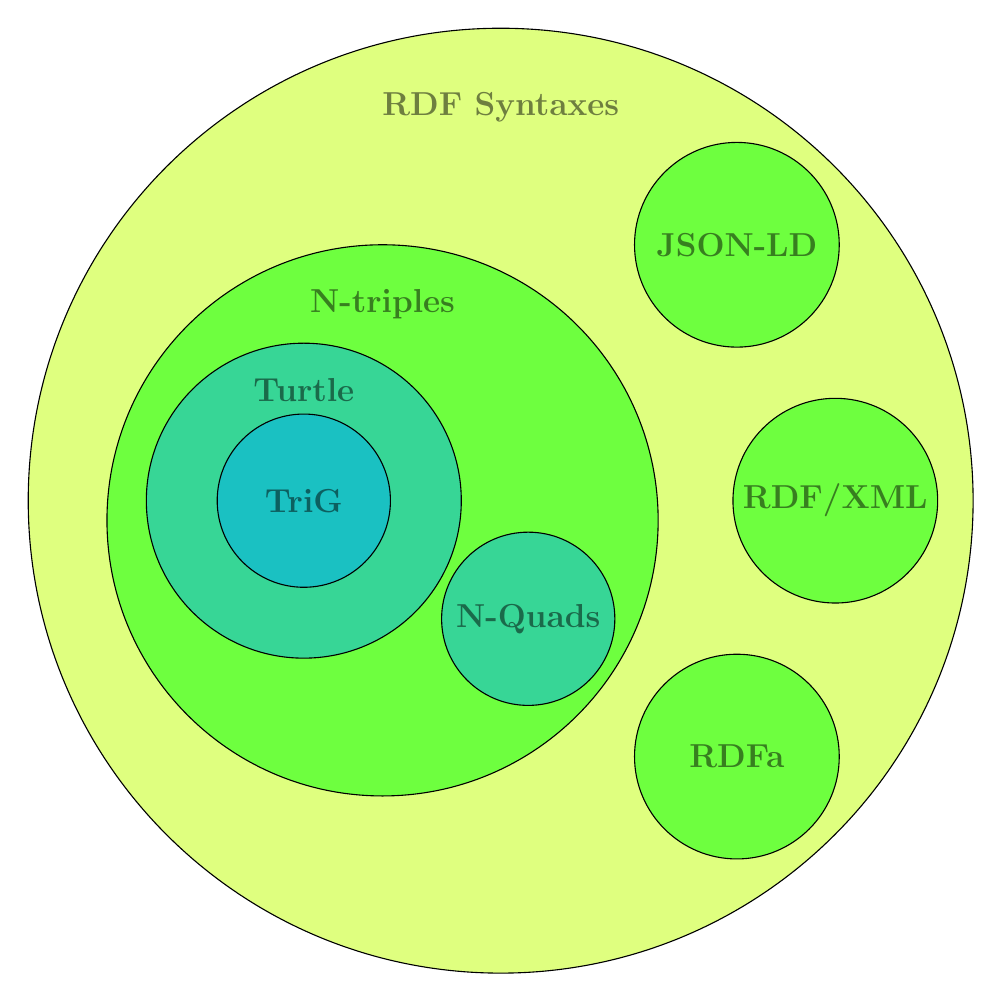
\begin{tikzpicture}
  \begin{scope}[shift={(3cm,-5cm)}, fill opacity=0.5]
    \draw[fill=lime, draw=black] (0,0) circle (6);
    \node at (0,5) (A) {\large\textbf{RDF Syntaxes}};

    \draw[fill=green, draw=black] (-1.5,-0.25) circle (3.5);
    \node at (-1.5,2.5) (C) {\large\textbf{N-triples}};
    \draw[fill=cyan, draw=black] (-2.5,0) circle (2);
    \node at (-2.5,1.4) (D) {\large\textbf{Turtle}};
    \draw[fill=cyan, draw=black] (-2.5,0) circle (1.1);
    \node at (-2.5,0) (H) {\large\textbf{TriG}};
    \draw[fill=cyan, draw=black] (0.35,-1.5) circle (1.1);
    \node at (0.35,-1.5) (I) {\large\textbf{N-Quads}};

    \draw[fill=green, draw=black] (3,3.25) circle (1.3);
    \node at (3,3.25) (E) {\large\textbf{JSON-LD}};

    \draw[fill=green, draw=black] (4.25,0) circle (1.3);
    \node at (4.25,0) (F) {\large\textbf{RDF/XML}};

    \draw[fill=green, draw=black] (3,-3.25) circle (1.3);
    \node at (3,-3.25) (G) {\large\textbf{RDFa}};
  \end{scope}
\end{tikzpicture}

RDFa extends existing markup with RDF triples.
This may be an \emph{alternative to content negotiation}.

\subsection{RDF Schema (RDFS)}

\emph{RDFS} is an RDF vocabulary
to model RDF vocabularies.

Practitioners often synonymize
vocabularies and \emph{ontologies}.
Strictly speaking, vocabularies are sets of words
while ontologies are \emph{sets of concepts and their relations}.

\subsection{Web Ontology Language (OWL)}

OWL extends RDFS with more advanced concepts.

\section{Querying and Reasoning}

\subsection{SPARQL}

SPARQL is a \emph{query language}
to manipulate RDF datasets.

The \emph{SPARQL protocol} is a Web API definition
for querying in the SPARQL language over HTTP.

The main building block of a SPARQL query is
a \emph{Basic Graph Pattern} (BGP).
A BGP is a set of \emph{triple patterns}.
A triple pattern is a triple
in which any component may be a variable.

A SPARQL query engine finds \emph{solution mappings}
such that the entire BGP is satisfied.

There are currently 4 read-only query forms.
\begin{itemize}
  \item \texttt{SELECT}: match values.
  \item \texttt{DESCRIBE}: match triples.
  \item \texttt{ASK}: check for existence.
  \item \texttt{DESCRIBE}: show information about a resource.
\end{itemize}

\subsection{RDFS, OWL and N3 inferencing}

\emph{Reasoning} allows clients
to combine knowledge from different sources
and infer facts.

\emph{RDFS reasoners} make entailments
based on RDFS semantics.
\emph{OWL reasoners} idem dito
based on OWL semantics.

For example, given the lines below.
\begin{lstlisting}
  <#Tim> foaf:knows <#Ted>.
  foaf:knows rdfs:domain foaf:Person.
\end{lstlisting}
An extra triple is created as follows.
\begin{lstlisting}
  <#Tim> a foaf:Person.
\end{lstlisting}

Rule-based reasoners allow users
to define their own rules.
An example is \emph{Notation3}
which allows additional constructs
such as variables, formulas or implications.
An example reasoner
which uses the Notation3 ruleset
is \emph{EYE}.

\chapter{Open Data}

\textit{Skip}.

\chapter{Video in the Web}

\section{Introduction: W3C's ``Video in the Web'' Activity}

There is a need for efficient adaptation
and rendering of multimedia.

In the example of a YouTube video;
the typical YouTube link represents a webpage.
The video is embedded into that webpage.
How to actually address the media source?

In addition, video has a time dimension.
How to refer to fragments of a video?

Since 2007, \emph{Video in the Web} is
one of 24 activities of the W3C.
Their mission is to make video
a \emph{first class citizen} of the Web.

\textit{
  Build a solid architectural foundation
  that enables people to create, navigate,
  search, link and distribute video,
  instead of an extension
  that doesn't take full advantage
  of the Web architecture.
}

\section{Addressing and annotating media fragments}

Example approaches may be
to add metadata in a seperate location
or to add a query or a fragment to the URI.

A good approach encompasses
\begin{itemize}
  \item independence of format,
  \item addressability of the temporal, spatial and track dimensions,
  \item the relation with the context,
  \item low complexity,
  \item minimal impact on the existing Web infrastructure,
  \item extraction of media in fragments.
\end{itemize}

The impact of server based fragment extraction.
\begin{itemize}
  \item Adaptations must be expressable in \emph{byte ranges}.
  \item Consequences for the axes
        \begin{itemize}
          \item \textbf{temporal}: intra-coded frames,
          \item \textbf{spatial}: necessity
                for independently coded spatial regions,
          \item \textbf{track}: identified by names or IDS.
        \end{itemize}
\end{itemize}

The temporal and track axes may be
easily expressed in terms of byte ranges.
Though, spatial fragments are very difficult
to express in terms of byte ranges.

\begin{tabular}{|c|c|}
  \hline
  fragment & query\\
  \hline
  \#t=20,30 & ?t=20,30\\
  \hline
  secundary resource (has context) & primary resource (no context)\\
  \hline
  adaptations must be expressable in byte ranges & no adaptation restrictions\\
  \hline
  fragments are not sent to server & key-value pairs are sent to server\\
  \hline
  maybe cacheable & not cacheable\\
  \hline
\end{tabular}

Fragments are \emph{resolved} by the user agent,
it may be translated to a \texttt{Range} header
and possibly an \texttt{Accept-Range-Redirect} header.

The toughest challenge is
to make current media sources
available via Media Fragments.

\section{Adaptive rendering of multimedia}

Under \emph{HTTP download-and-play} a media resource is
downloaded and played upon completion.

Under \emph{HTTP progressive download} a media resource is
downloaded and as soon as
a certain amount has been received,
playback already starts.

Under \emph{real-time streaming} a media resource is
sent at about the same rate it plays.
This protocol is stateful.
This dates back to the times
of \emph{RealPlayer} and such.

There are pros and cons
to HTTP and real-time approaches.
\emph{HTTP adaptive streaming} combines
best of both worlds.
Except server-side monitoring.

Media resources are divided into \emph{chunks},
typically 2-10 seconds.
Each chunk starts with a random access point.
There is no need
for physically separated segments.
The chunks are housed in a container format.

A media resource is represented
by a manifest and its chunks.
A manifest contains information
about versions and segments.
Any chunk is adressable
by a HTTP request.

The client reads the manifest, then proceeds
to steer the media delivery himself (pull vs. push).

Apple specifies this as \emph{HTTP Live Streaming}.
Their specification is independent of container format.
The format of their manifest is M3U8.

Microsoft specifies \emph{Smooth Streaming}.
It works only with \emph{fragmented MP4 files}.
Their manifest is an XML-based proprietary format.
Chunks are addressed by unique \emph{URIs}.

Adobe's \emph{HTTP Dynamic Streaming} works
with fragmented MP4 files
and only through a Flash media server
(or extended Apache server).
Their manifest is in an XML-based proprietary format.
Chunks are addressed by \emph{byte ranges}.

The master specification is
\emph{Dynamic Adaptive Streaming over HTTP} (DASH).
In principle it doesn't depend on anything.
The manifest is highly flexible
with regard to the organisation of chunks.
Both byte ranges and physically separated files are possible.

\section{Content networks}

\textit{Skip}.

\end{document}